\section{Protocollo SETA}

	Il protocollo SETA (SEcure sharing of TAsks in clustered wireless sensors networks) nasce al fine di garantire sicurezza e privacy all'interno delle rete di sensori, senza sacrificare il risparmio energetico.
	La principale caratteristica che caratterizza e distingue SETA è l'adozione di un'architettura ibrida (wireless sensors network, wireless mesh network), i nodi sensori sono organizzati in cluster e comunicano con i cluster heads, i quali sono i router in grado di comunicare con la sink (Figura \ref{fig:architetturaReteSETA}).
	SETA mira a fornire integrità dei dati, anonimato, risparmio energetico e aggregazione dei dati sicura di tipo end-to-end.
	
	\begin{figure}[h]
		\centering
		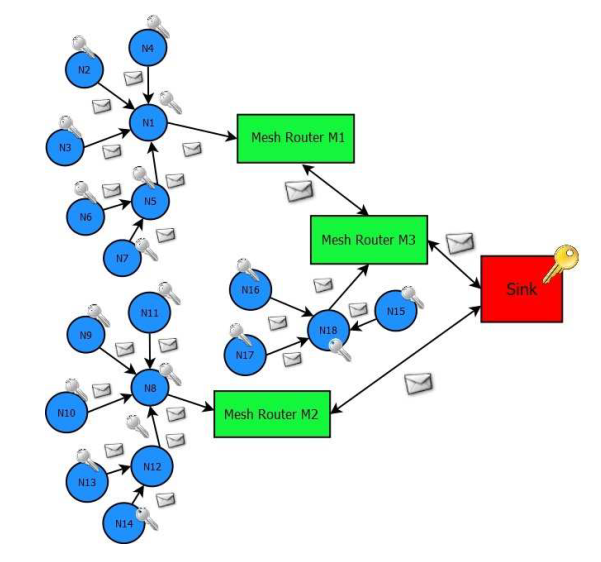
\includegraphics[width=0.5\textwidth]{lez6-SETA/SETA_NetworkModel.png}
		\caption{Architettura di rete del protocollo SETA}
		\label{fig:architetturaReteSETA}
	\end{figure}
	
\paragraph{Aspetti chiave}
	Condivisione dei compiti sulla base delle diverse disponibilità energetiche e capacità computazionali tra sensori e cluster head.
	I nodi sensori svolgono il ruolo di soggetto e processore, si occupano solamente di registrare il dato e criptarlo;
	i cluster head svolgono il ruolo di soggetto nell'aggregare i dati, di processore nella criptazione dei dati e di controller nella verifica dell'integrità dei dati ricevuti.
	
\paragraph{Procedura di trasmissione}
	\begin{enumerate}
		\item I nodi sensori acquisiscono i dati dall'ambiente, li criptano e li inviano al CH
		\item Ogni CH attraversato verifica l'integrità dei dati
		\item La sink decifra i dati e genera le statistiche
	\end{enumerate}

	La verifica di integrità è svolta dal CH nel seguente modo:
	in caso di violazione della privacy viene inviata alla sink una notifica di errore,
	altrimenti il dato può essere aggregato o meno a seconda del livello di congestione della rete e inviato alla sink.\\
	L'assegnamento del ruolo di controllore di sicurezza ai CH riduce il traffico sulla rete e di conseguenza l'overhead, con un sensibile risparmio energetico.
	Gli aspetti negativi della congestione di rete sono lo spreco energetico e la compromissione dell'accuratezza delle stime.
	Ogni qual volta il numero di messaggi del buffer in trasmissione supera una certa soglia, il CH aggrega i dati al fine di evitare l'overflow del buffer; l'aggregazione dei dati è possibile senza che i messaggi vengano decriptati grazie a un algoritmo di \emph{homomorphic enryption}.
	
	 %possibile inserire dettagli sulla struttura del messaggio
	 
\paragraph{Valuzione delle prestazioni}
	In simulazione SETA è stato confrontato con DyDAP: in condizioni ideali DyDAP presenta prestazione migliori, situazione che però si inverte in presenza di nodi malevoli, dove SETA è in grado di generare un minor carico sulla rete;
	SETA è in grado di garantire una maggior accuratezza dei dati in seguito ad aggregazione; 
	DyDAP presenta un leggere vantaggio nei tempi di consegna dei messaggi alla sink;
	SETA garantisce un consumo energetico sensibilmente inferiore.
	
	
	
	
	
	
	
	
	
	
	

	